Figure~\ref{fig:broom10} shows where the loss occurs on a held-out frame. C breaks up the continuous pavement around the broom and introduces high-contrast streaks across the ground. U recovers the pavement boundary and broom silhouette, although the bristles and fine pavement texture remain softer than the reference. The whole-frame PSNR is 12.74~dB for C, 19.06~dB for U and 23.11~dB for the full source.
\begin{figure}[!htbp]\centering
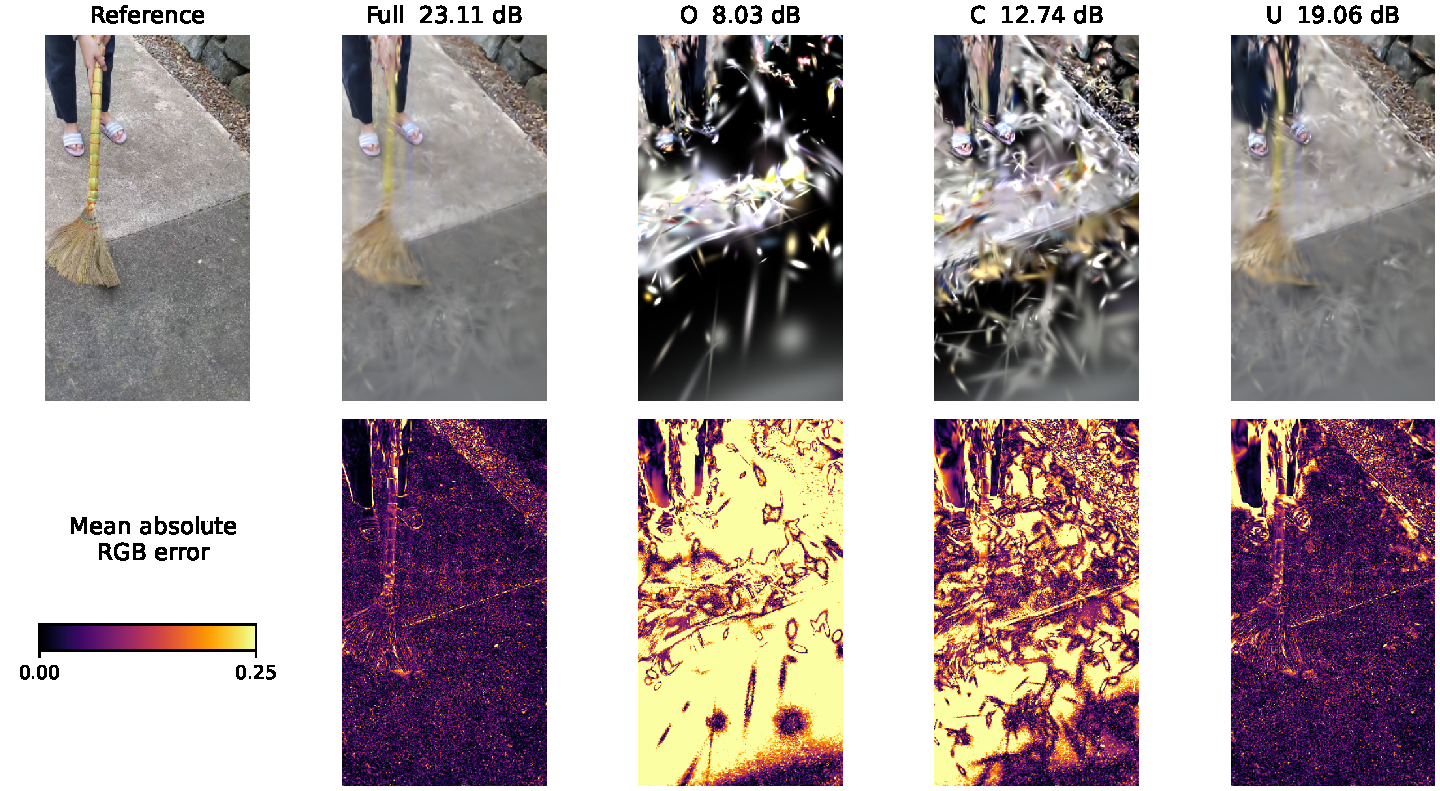
\includegraphics[width=\linewidth]{broom_10.pdf}
\caption{Ordinary Broom at 10\% retention (seed zero, 7,886 of 78,863 points). From left to right: reference image, full source, opacity (O), restricted influence (C) and unrestricted influence (U). Each label is whole-frame PSNR against the reference. The lower row shows mean absolute RGB error on the same linear scale, clipped at 0.25 on $[0,1]$ images. We chose the middle of the 197 held-out frames by list position (zero-based index 98), independently of frame quality.}\label{fig:broom10}\end{figure}
